%\documentclass[notes]{beamer}       			% compila sia i frame che le note
\documentclass{beamer}              			% compila solo i frame
%\documentclass[notes=only]{beamer}  	% compila solo le note

% ita language and encoding
\usepackage[utf8]{inputenc}
\usepackage[italian]{babel}

% formattazione
\usepackage{ragged2e} 							% pacchetto che contiene il comando \justifying
\apptocmd{\frame}{}{\justifying}{}  	% --> applica la giustificazione a tutti i frame del documento
%\justifying											% --> applica la giustificazione a tutto il documento

% graphics style
\usepackage{graphicx}
\usepackage{xcolor}
\usepackage{shadowtext}

%image paths
\graphicspath{{./Immagini/}}

% impostazioni base delle slide - tema, colori, caratteri, ... (deic.uab.es/~iblanes/beamer_gallery/)
\mode<presentation>
{
	\usetheme{CambridgeUS}      % or try Darmstadt, Madrid, Warsaw, ...
  	\usecolortheme{rose} 			% or try albatross, beaver, crane, orchid, rose ...
	\usefonttheme{structurebold} % or try structureitalicserif, structuresmallcapsserif
}

% settagio dati principali del file - titolo, autore, ...
\title[University of Perugia]{The AMS-02 experiment}
\subtitle{General review of the apparatus}
\author{Daniele Di Bari}
\date{27th April 2017}

% settaggio prima slide
\setbeamertemplate{title page}
{
	\shadowcolor{white!30!black}
	\vspace{-0.5cm}	
	
    \shadowtext{\textcolor{white}{\textbf{\footnotesize{The Alpha Magnetic Spectrometer}}}}
   
    \vspace{0.15cm}  	
    
   	\shadowtext{\textcolor{white}{\textbf{\LARGE \inserttitle}}}\par
      
   	\vspace{0.1cm}  

   	\shadowtext{\textcolor{white}{\emph{\large \insertsubtitle}}}\par
   	
   	\vspace{2.5cm}
	
	\titlepagetext{lightgray}{The general particle physics}\\
	\titlepagetext{lightgray}{experiment in space, on board}\\
	\titlepagetext{lightgray}{the International Space Station}\\
	\titlepagetext{lightgray}{since 19th May 2011.}		
}
				
% colors
\definecolor{itemred}{RGB}{163,0,0}
\definecolor{itemblue}{RGB}{52,57,176}

% COMANDI
% Formato testo generico in titolpage
\newcommand\titlepagetext[2]{\textcolor{#1}{\footnotesize{\textit{{#2}}}}}
\newcommand\colortextbf[2]{\textcolor{#1}{\textbf{#2}}}
\newcommand\bluetextbf[1]{\textcolor{itemblue}{\textbf{#1}}}
% Testo giustificato
\newenvironment<>{justify}{\justifying{}}

\begin{document}
	% impostare una foto come sfondo del frame: 
	\usebackgroundtemplate{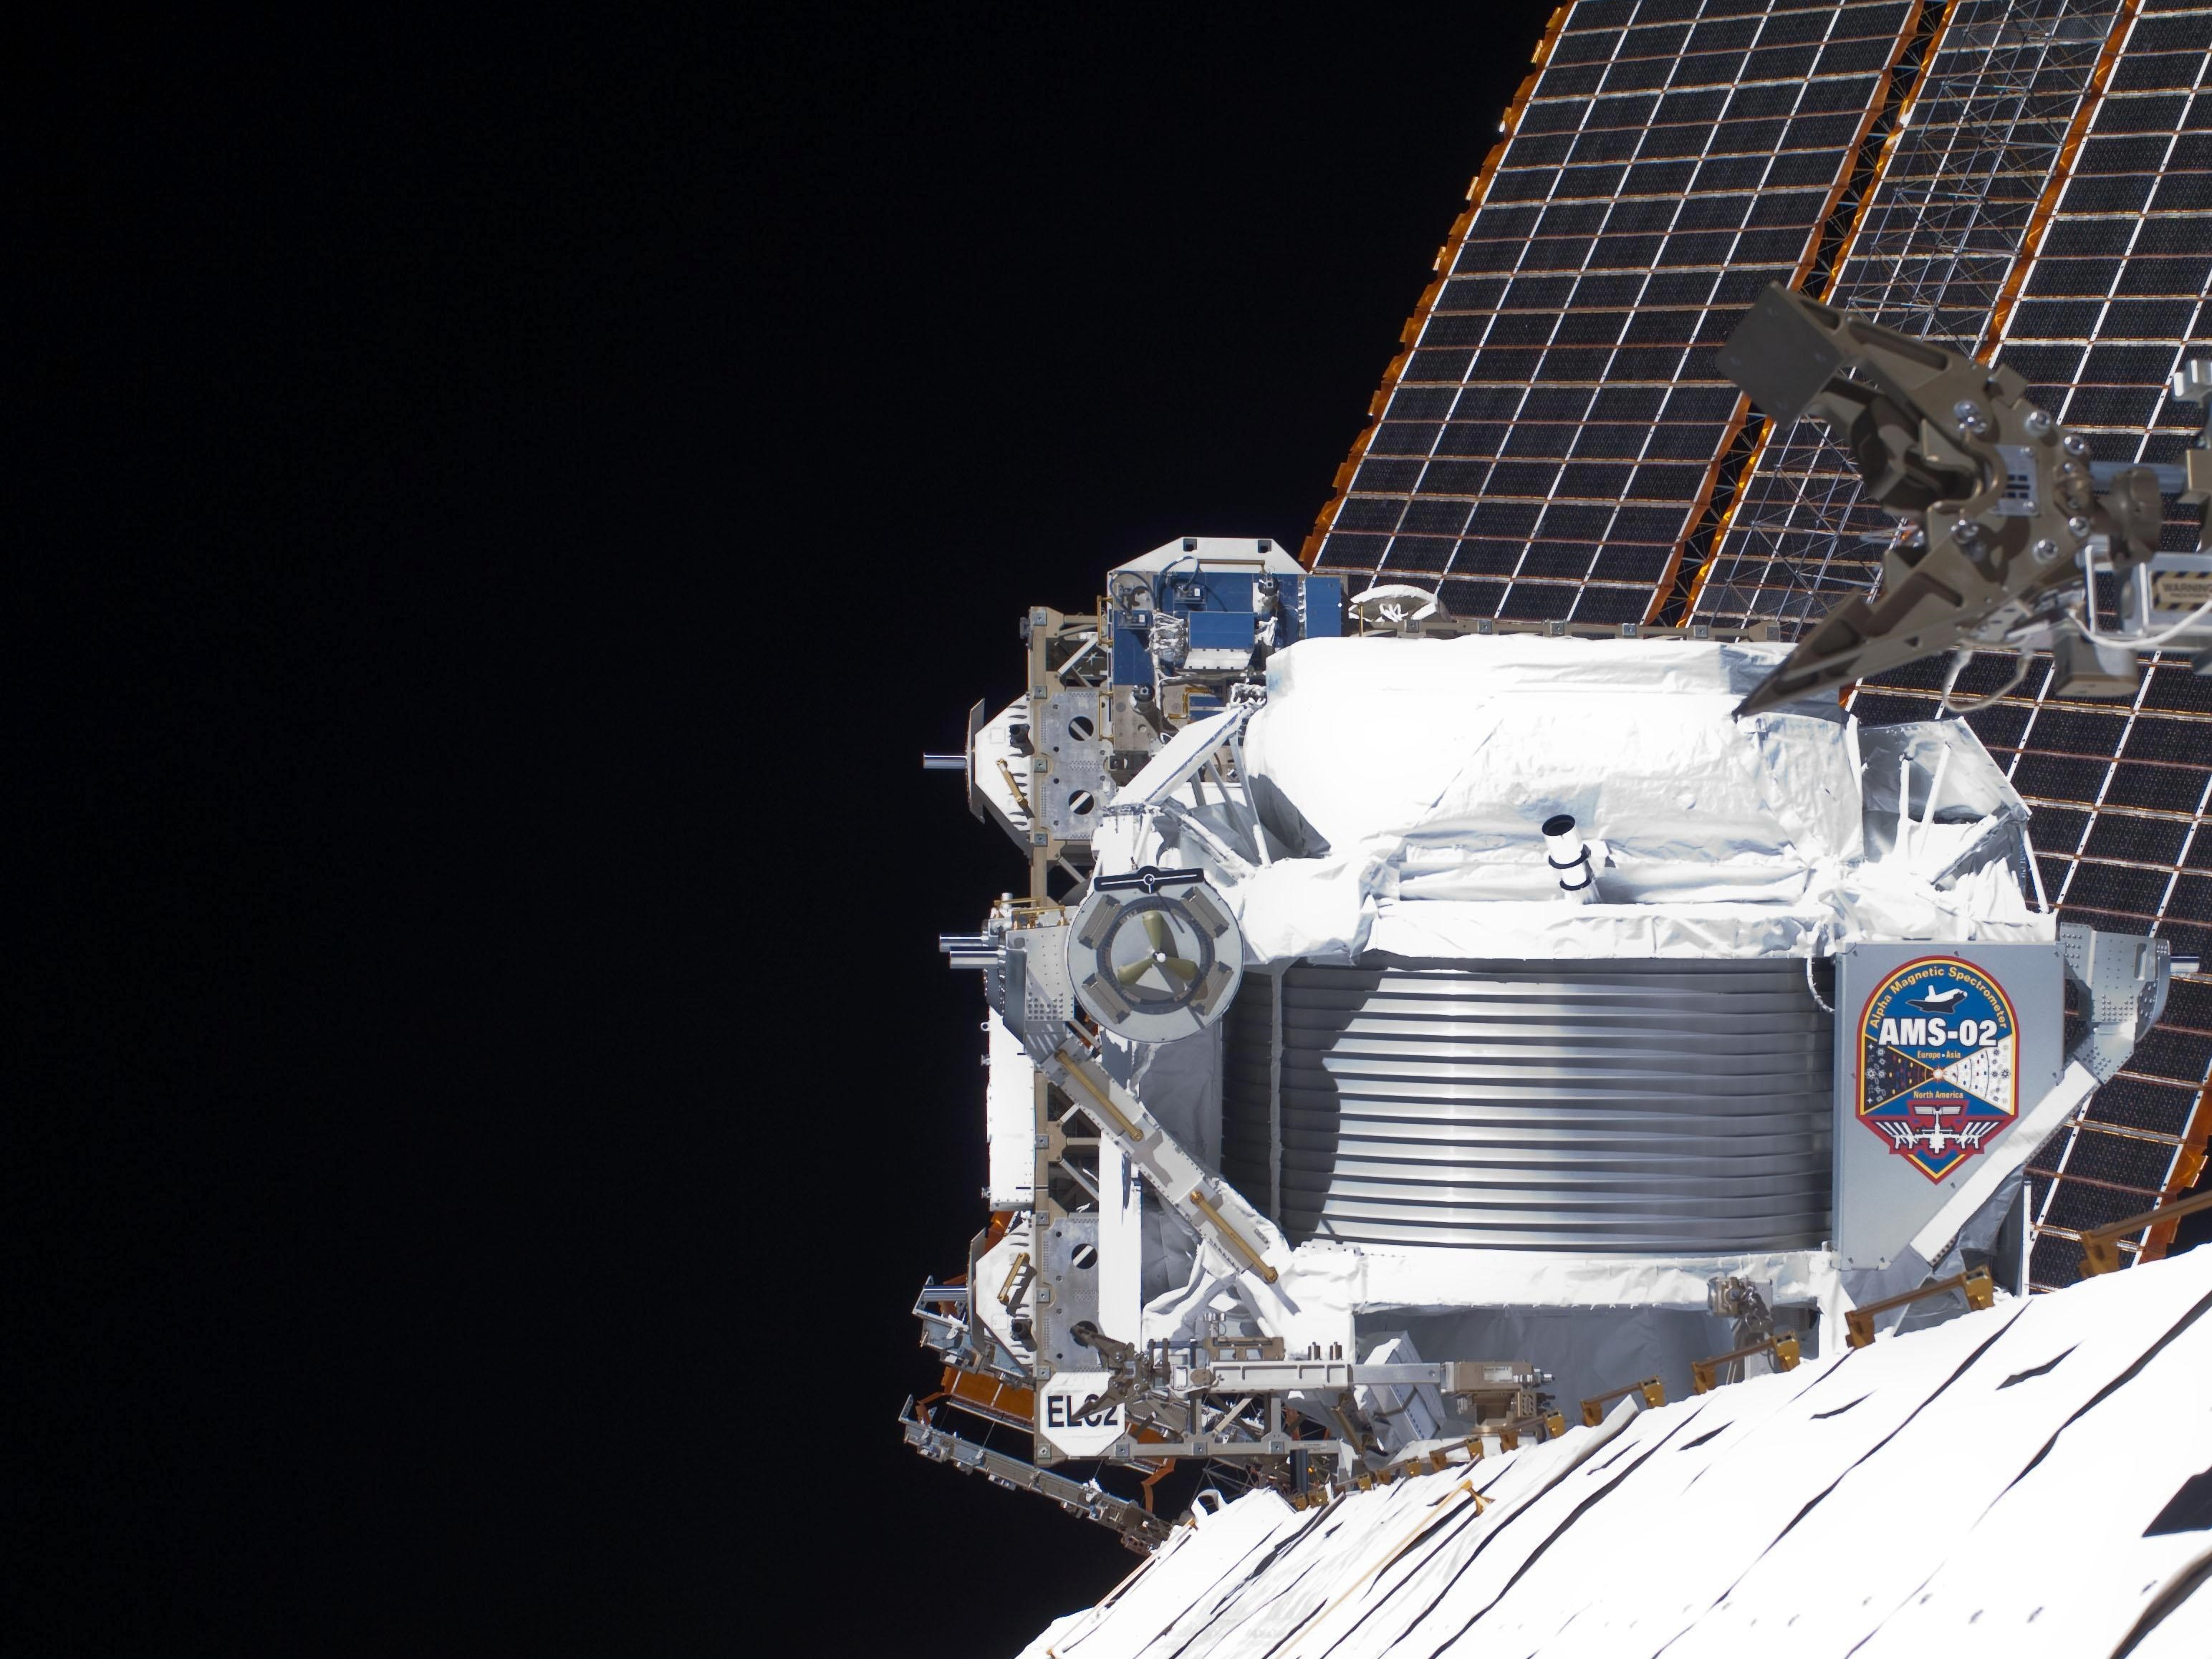
\includegraphics[height=\paperheight,keepaspectratio]{on_ISS-08_cutMIDDLEUP-3088.jpg}}	
	% 	possibili impostazioni per l'img: width=\paperwidth  --  height=\paperheight  --  keepaspectratio

\section{Course of Particle Detectors}
\subsection{Presentation on the AMS-02 experiment}

\begin{frame}
	\titlepage
\end{frame}

\note{ 
   ciao
}

\usebackgroundtemplate{}

%\begin{frame}
%	\frametitle{Technical Question about the Detector}
%	AMS is a particle physics experiment in space, so it focuses on the detection of particles, but:
%	\begin{itemize}
%	\item	Which kind of particle do we have to detect?
%	\item	What is the required dimension of the detector?
%	\item	Which ``property'' of the particle do we have to know?
%	\begin{itemize}
%		\item[$\circ$]	Position - Trajectory
%		\item[$\circ$]	Time
%		\item[$\circ$]	Number
%		\item[$\circ$]	Energy
%		\item[$\circ$]	Momentum
%	\end{itemize}
%	\item	What is the required resolution?
%	\item	What is the maximum count rate?
%	\item	What is the time distribution of the events?
%	\item	And last, but not least, how much does it cost? 
%	\end{itemize}
%\end{frame}

\begin{frame}
\frametitle{Index}

Inserire la scaletta della presentazione
\end{frame}

\begin{frame}
	\setbeamertemplate{background}{white}
	\frametitle{Introduction}
	\framesubtitle{The Alpha Magnetic Spectrometer}
	AMS-02 is a general purpose \textbf{high energy particle detector.}
	
	\vspace{0.25cm}
	\begin{block}{Purpose of the AMS experiment}
		\justifying
		To perform accurate, high statistics, long duration measurements of the spectra of energetic primary charged 
		cosmic rays in space. 
	\end{block}
		
	\vspace{0.25cm}
	Some of the \textbf{physics goals} are:
	\begin{enumerate}
		\item \bluetextbf{Dark Matter}
		\item \bluetextbf{Matter/Antimatter Asymmetry}
		\item \bluetextbf{Cosmic Ray Physics}
	\end{enumerate}
\end{frame}
\note{
	AMS-02 (Alpha Magnetic Spectrometer ) is a general purpose high energy particle detector which was successfully deployed on 
	the International Space Station (ISS) on May 19, 2011 to conduct a unique long duration mission of fundamental physics 
	research in space. Among the physics objectives of AMS are the searches for an understanding of Dark Matter, Anti-matter, the 
	origin of cosmic rays and the exploration of new physics phenomena not possible to study with ground based experiments
	Lo scopo dell'esperimento è quello di effettuare, per un periodo di lunga durata così da ottenere un'elevata statistica, delle 
	misure molto accurate dello spettro di energia (per energie fino all'ordine dei TeV) dei raggi cosmici carichi primari direttamente 
	nello spazio.
}

\begin{frame}
    \frametitle{Technical Requirements}
    \framesubtitle{From Physics Goals}
    
	Physical goals involve \textbf{technical requirements for the AMS detector}:
	
	\begin{itemize}
		\item	\bluetextbf{Dark Matter $\Rightarrow$}
					to get $e^+/p$ rejection of $\sim10^{-6}$ for the measurement of the positron fraction.
		\item	\bluetextbf{Matter/Antimatter Asymmetry $\Rightarrow$}
					to reach a sensitivity in the search for anti-matter nuclei of $10^{-10}$ (ratio of anti-helium nuclei to helium nuclei).
		\item	\bluetextbf{Cosmic Ray Physics $\Rightarrow$}
					to measure the composition and spectra of charged particles with an accuracy of 1\%.
	\end{itemize}
	
	Moreover, \bluetextbf{for each of these ones}, it is very important to extend, as far as possible, the energy range of the 
	measurements.
	
	For AMS, the required energy range is from 0.5 to $\sim$ 2000 $GeV$.

	%\footnotesize{\underline{\textbf{Note}} These requirements represent a considerable sensitivity improvement compared to the previous space-borne experiments.}

\end{frame}

\note{
	Esiste un forte interesse nell'effettuare delle misure di precisione della frazione di positroni dei raggi cosmici nella regione 
	energetica da 10 a 1000 GeV, in quanto le misurazioni di $e^+ / (e^+ + e^-)$, da AMS-01, HEAT, PAMELA e FERMI indicano 
	una grande deviazione di questo rapporto dalla produzione di e+ e e- previsto da un modello che comprende solo collisioni ordinarie del raggio cosmico.
   	 
   	These available measurements are both at too low an energy and of too limited statistics to shed the light on the origin of this 
   	significant excess.
   	 
	AMS-02 is expected to provide definitive answers concerning the nature of this deviation.
}

\begin{frame}
	\frametitle{Technical Requirements}
    \framesubtitle{From Physics Goals}	
    
    \begin{block}{The technical challenge of AMS-02}
		\justifying
		The illustrated requirements represent a considerable sensitivity improvement compared to the previous space-borne 
		experiments.
	\end{block}
   	
   	\vspace{0.25cm}
	\small{\bluetextbf{NOTE}}
	\vspace{-0.2cm}
    \begin{itemize}
    	\item[\footnotesize{$\blacktriangleright$}] 
    		\footnotesize{There is a strong demand for precision measurements of cosmic rays in the energy region from 10 to 1000 
    		$GeV$ as the measurements of positron fraction, i.e.  $e^+ / (e^+ + e^-)$, by AMS-01, HEAT, PAMELA and FERMI 
    		indicate a large deviation of this ratio from the production of $e^+$ and $e^-$ predicted by a model that includes only 
    		ordinary cosmic ray collisions.
    		
    		These available measurements are both at too low an energy and of too limited statistics to shed the light on the origin of 
    		this significant excess.
    		
    		AMS-02 is expected to provide definitive answers concerning the nature of this deviation.}
   	\end{itemize}  
   	 
%
%%	\vspace{0.25cm}
%	There is a strong demand for precision measurements of cosmic rays in the energy region from 10 to 1000 GeV as the 
%	measurements of e+/(e+ + e-) by AMS-01, HEAT, PAMELA and FERMI indicate a large deviation of this ratio from the 
%	production of e+ and e- predicted by a model that includes only ordinary cosmic ray collisions. 
%	
%	These available measurements are both at too low an energy and of too limited statistics to shed the light on the origin of this 
%	significant excess. 
%	
%	AMS-02 is	expected to provide definitive answers concerning the nature of this deviation.
\end{frame}

%\begin{frame}
%	\frametitle{Technical Requirements}
%    \framesubtitle{From Physics Goals}
%	\begin{columns}
%		\begin{column}{0.5\textwidth}
%			\begin{center}
%				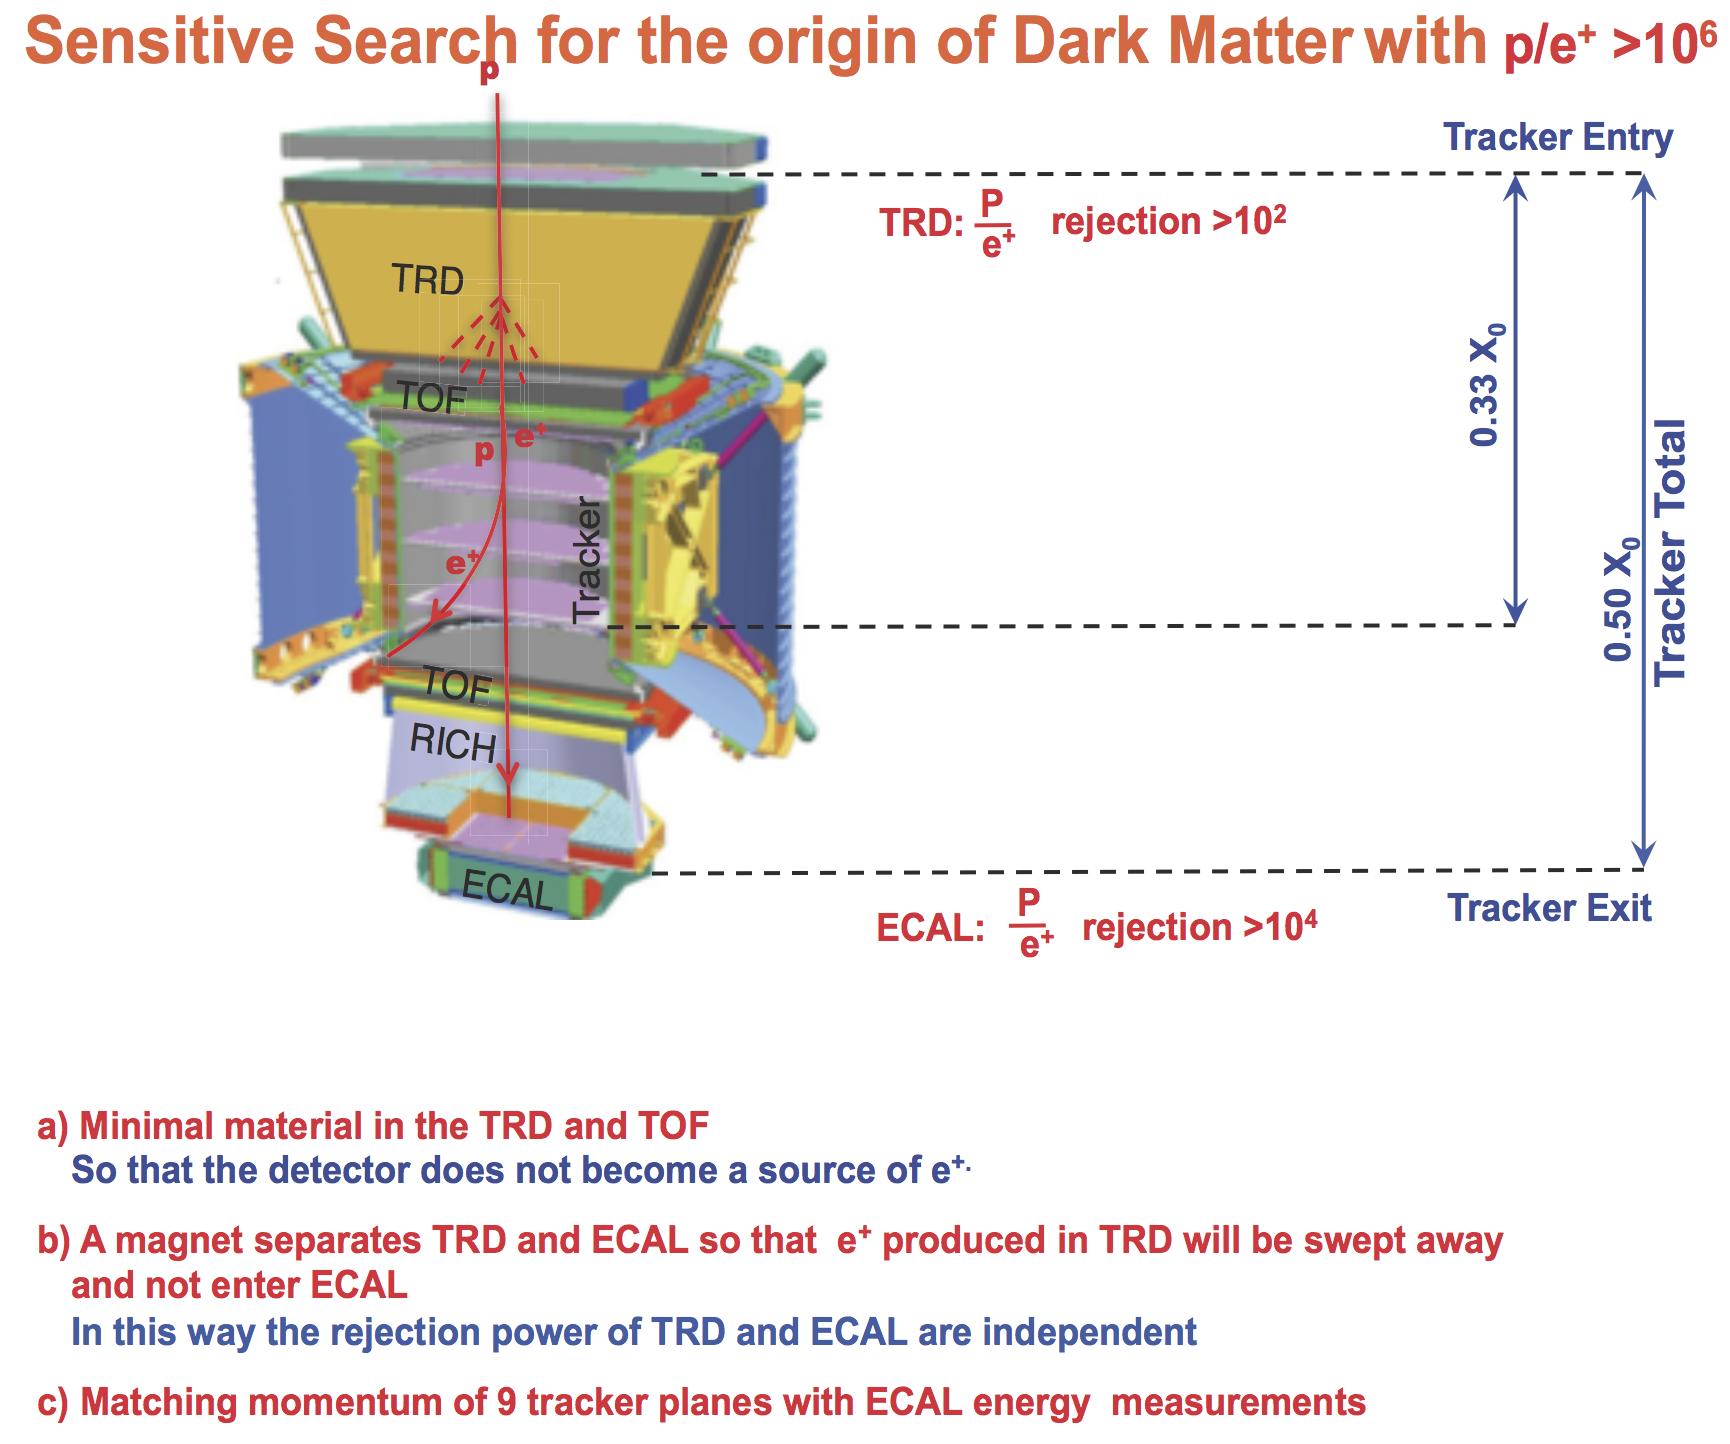
\includegraphics[width=0.95\columnwidth]{Schem_Requirements-DM.png}
%			\end{center}
%		\end{column}
%
%		\begin{column}{0.5\textwidth}
%			\begin{center}
%				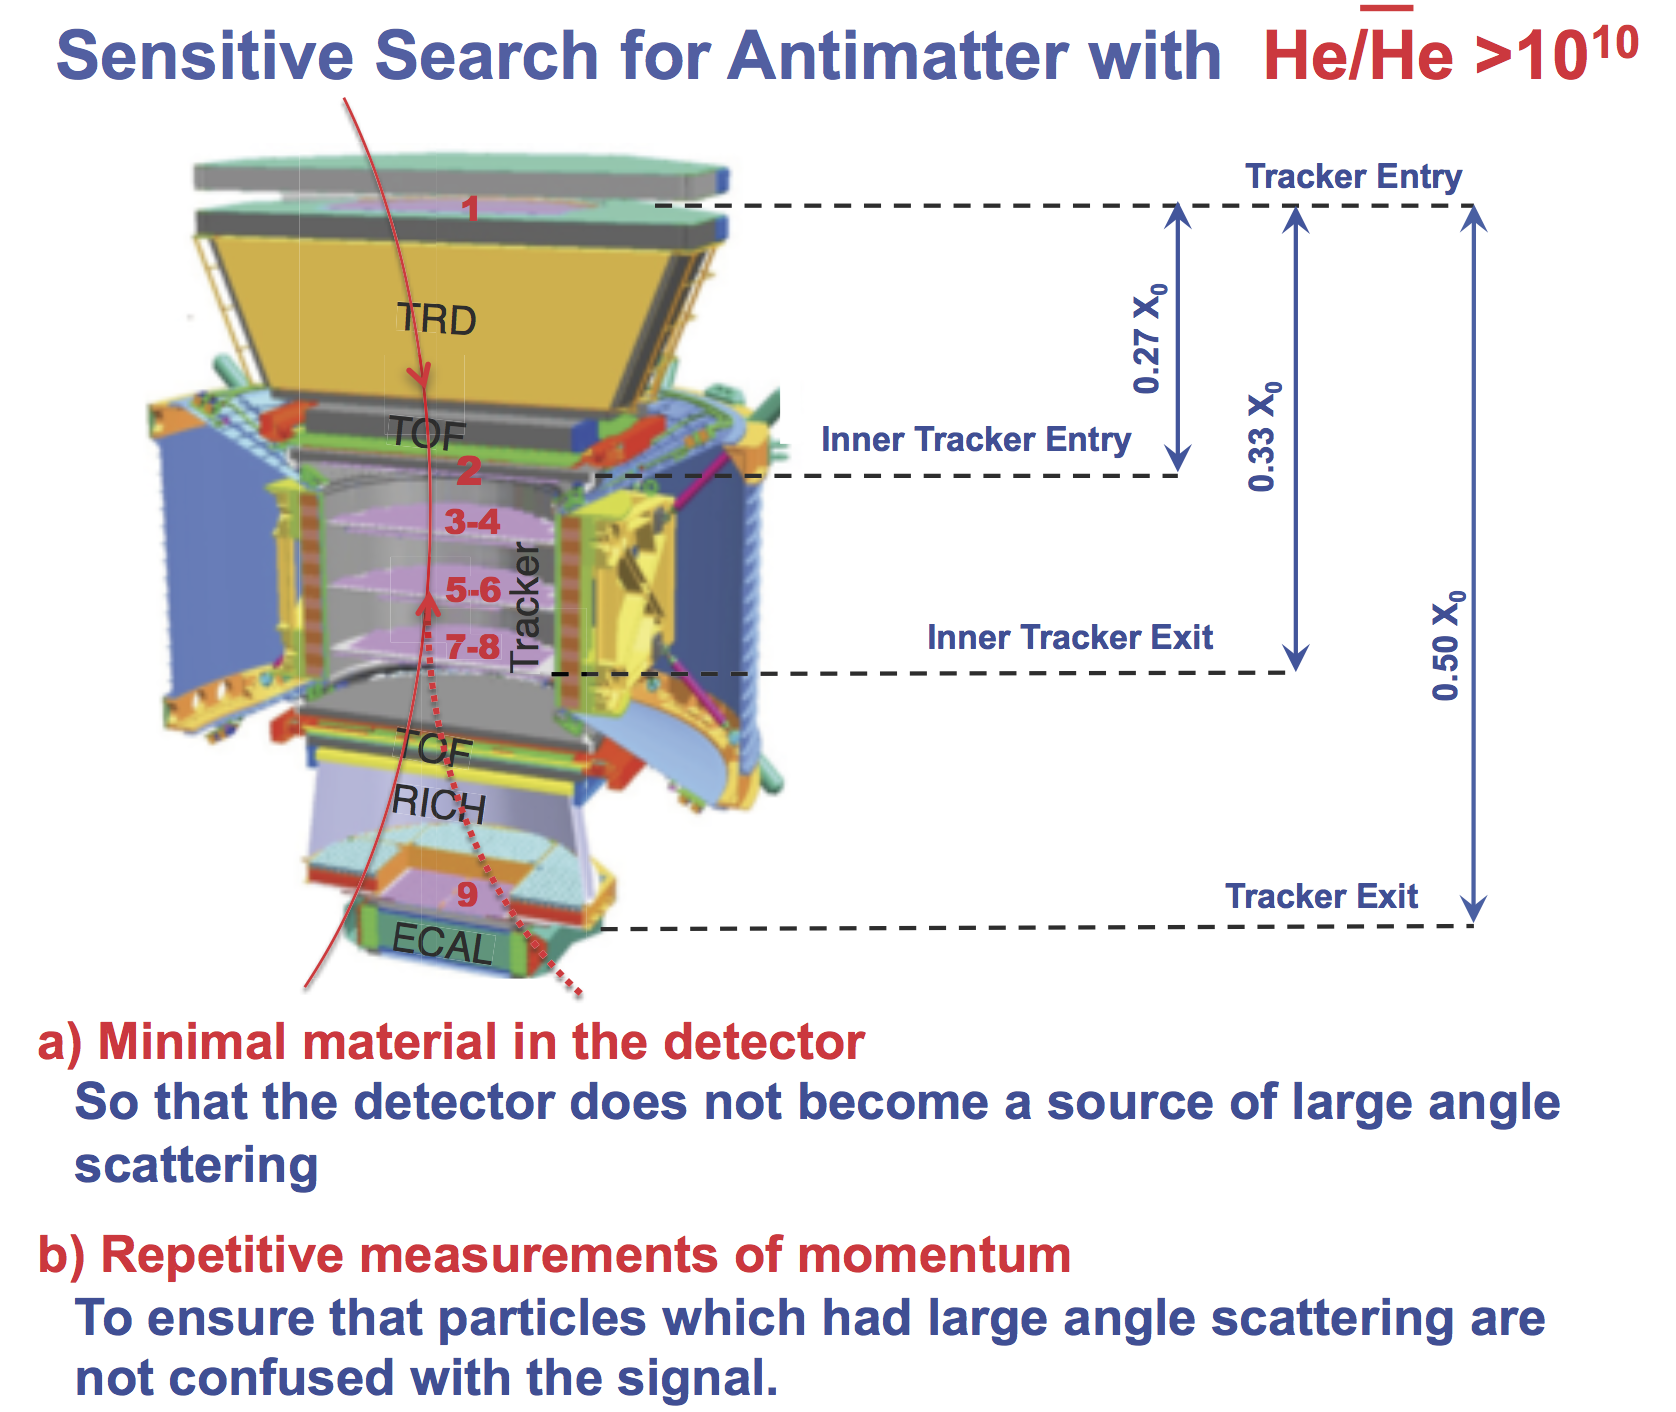
\includegraphics[width=0.95\columnwidth]{Schem_Requirements-Antimatter.png}
%			\end{center}
%		\end{column}
%	\end{columns}
%\end{frame}

\begin{frame}
	\frametitle{Technical Requirement}
	\framesubtitle{General structure of the AMS apparatus}
	\begin{center}
		\vspace{-0.45cm}
		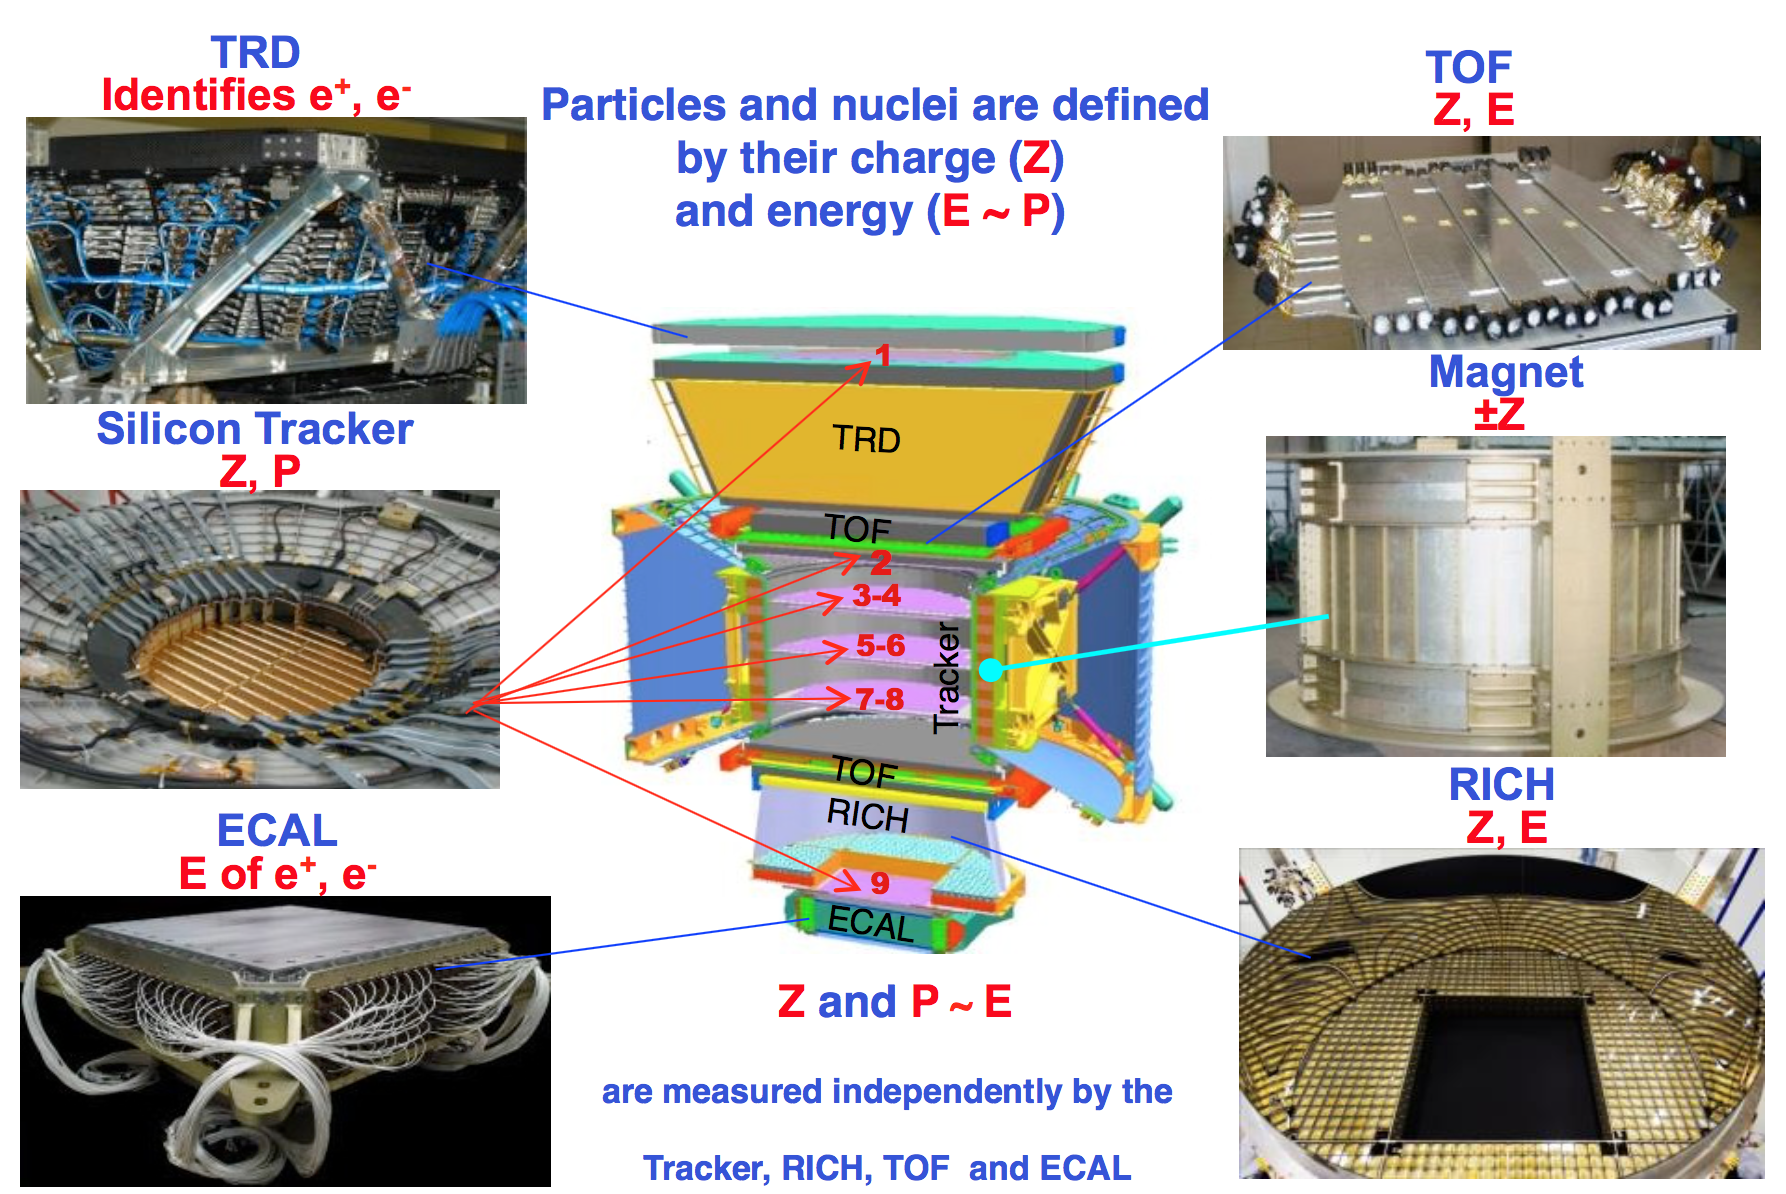
\includegraphics[height=0.7\paperheight]{Schem_structure_of_AMS-02.png}
	\end{center}
\end{frame}

\begin{frame}
	\frametitle{Technical Requirement}
	\framesubtitle{From the research on the Dark Matter}
	\begin{center}
		\vspace{-0.1cm}
		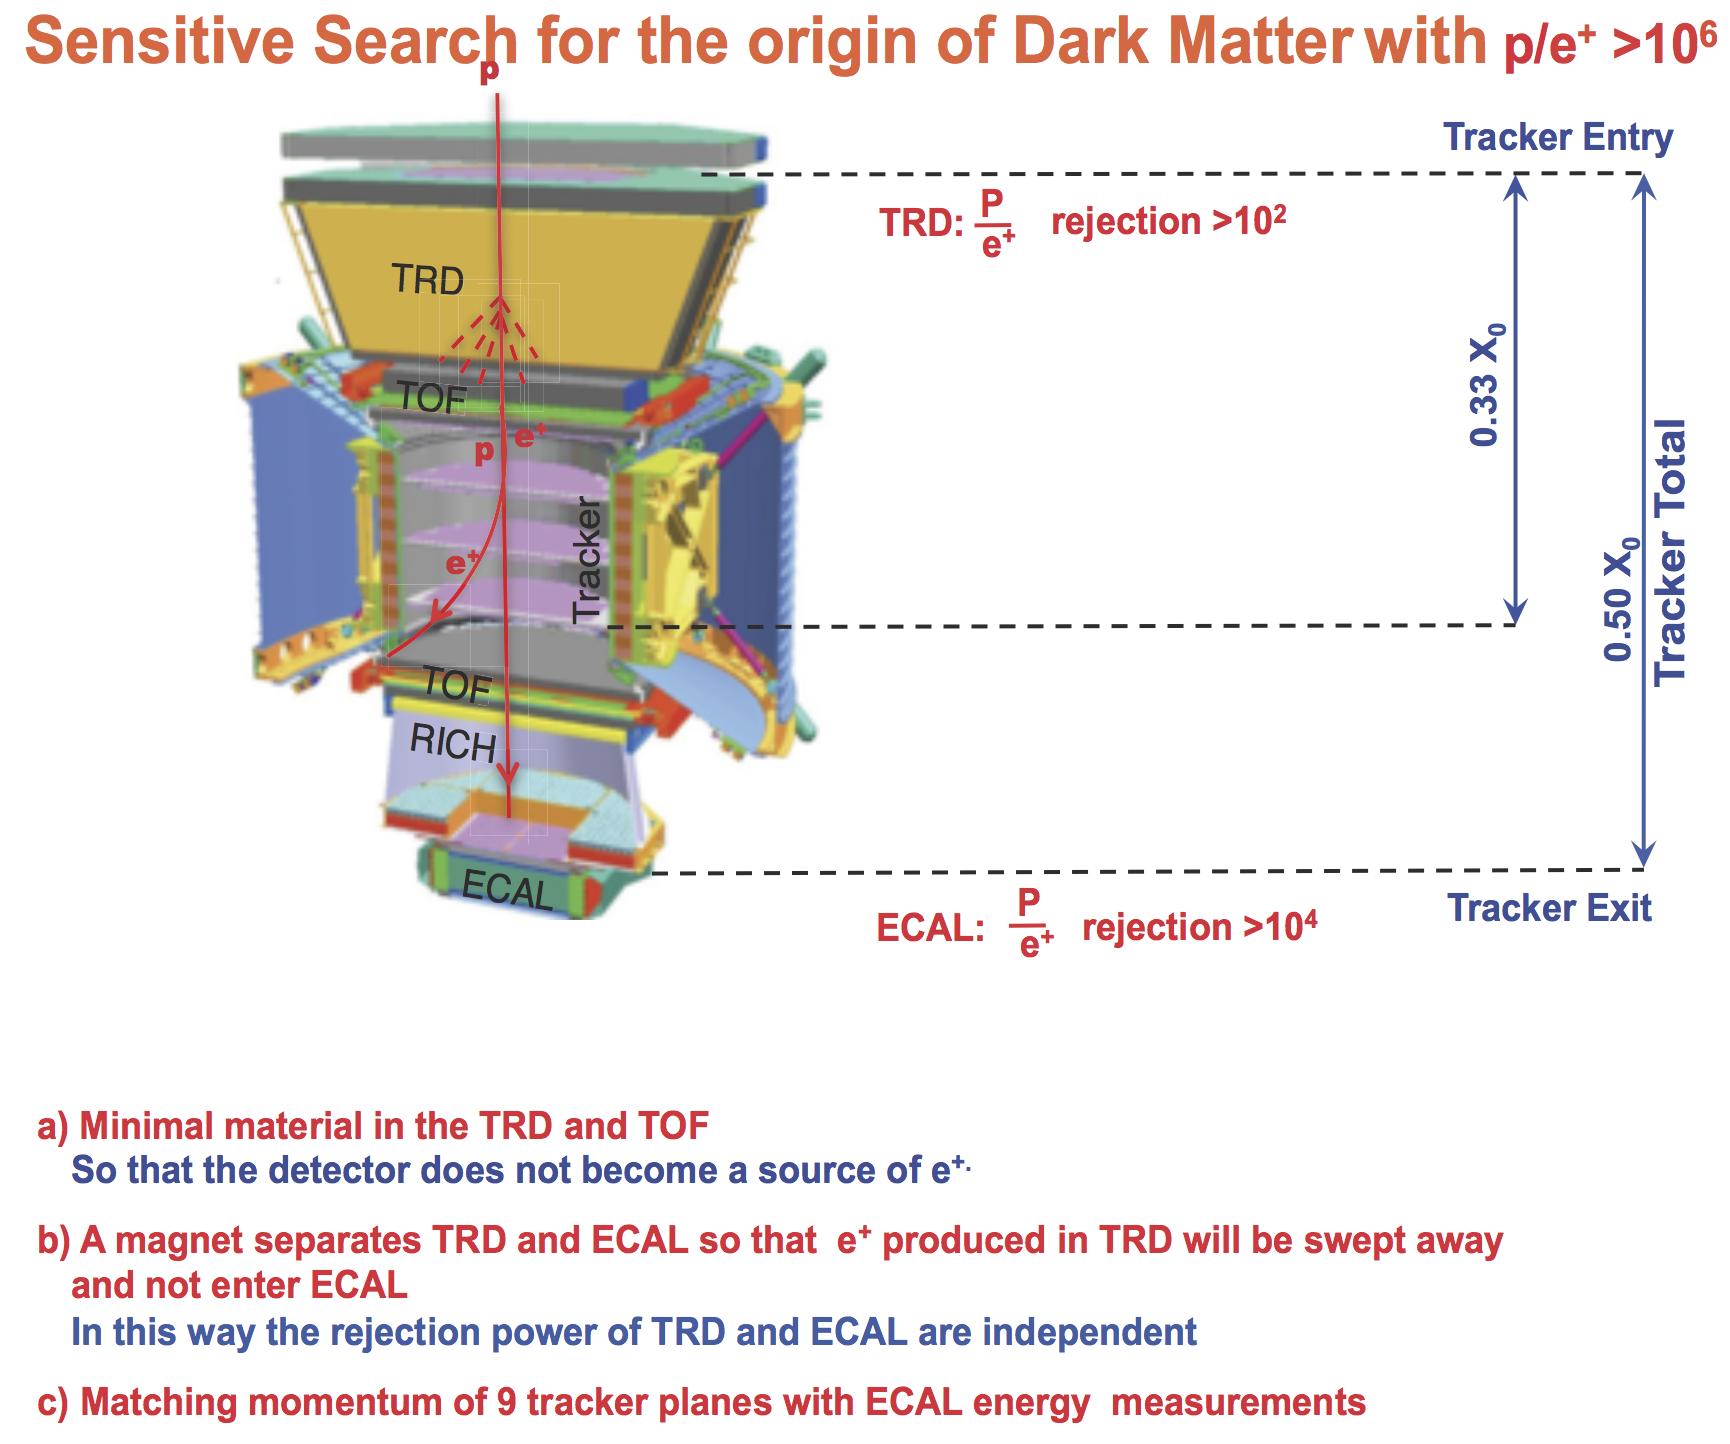
\includegraphics[height=0.72\paperheight]{Schem_Requirements-DM.png}
	\end{center}
\end{frame}

\begin{frame}
	\frametitle{Technical Requirement}
	\framesubtitle{From the research on the Matter/Antimatter Asymmetry}
	\begin{center}
		\vspace{-0.1cm}
		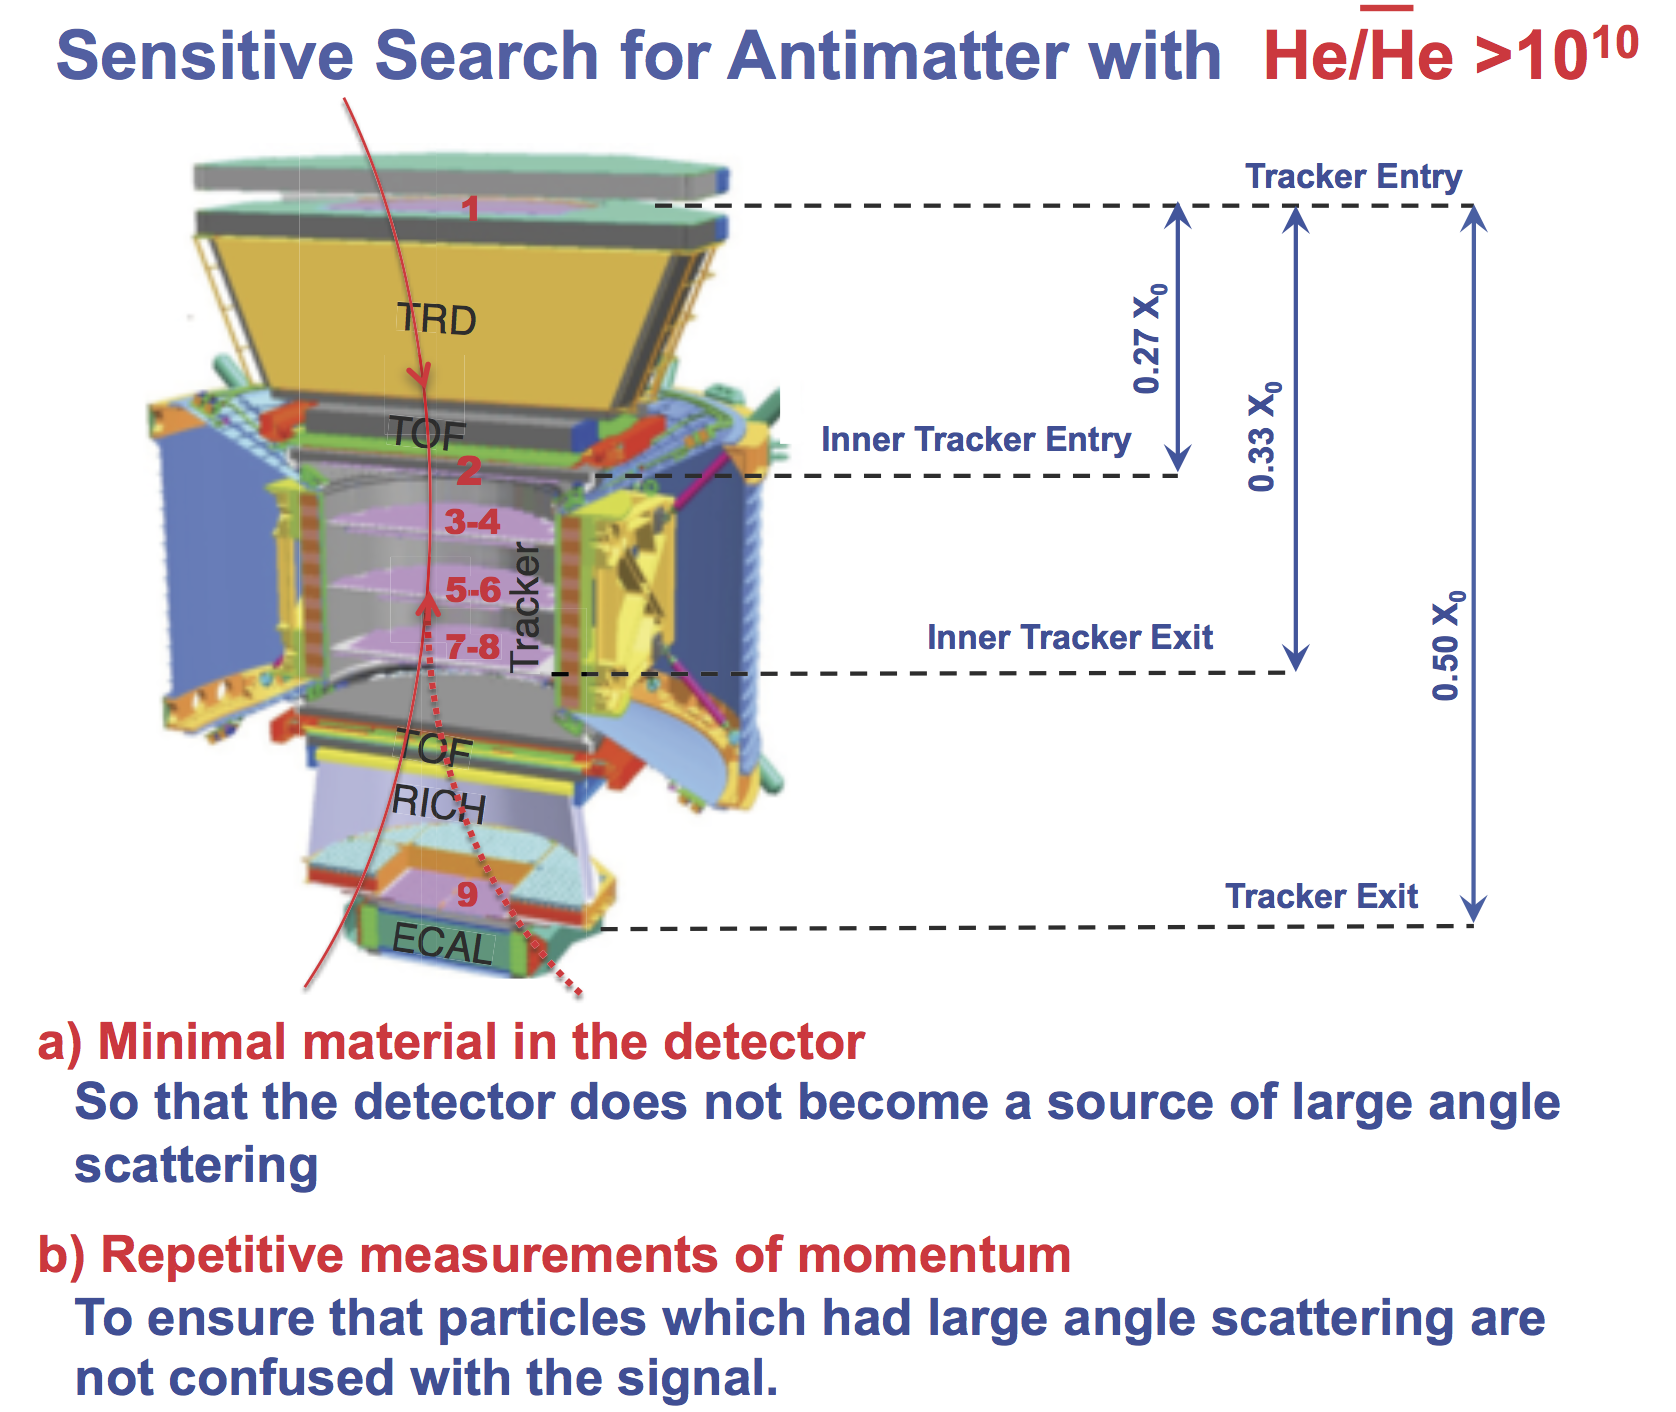
\includegraphics[height=0.65\paperheight]{Schem_Requirements-Antimatter.png}
	\end{center}
\end{frame}

\begin{frame}
	\frametitle{Technical Requirement}
	\framesubtitle{From the research on the Cosmic Ray}
	\begin{center}
		\vspace{-0.5cm}
		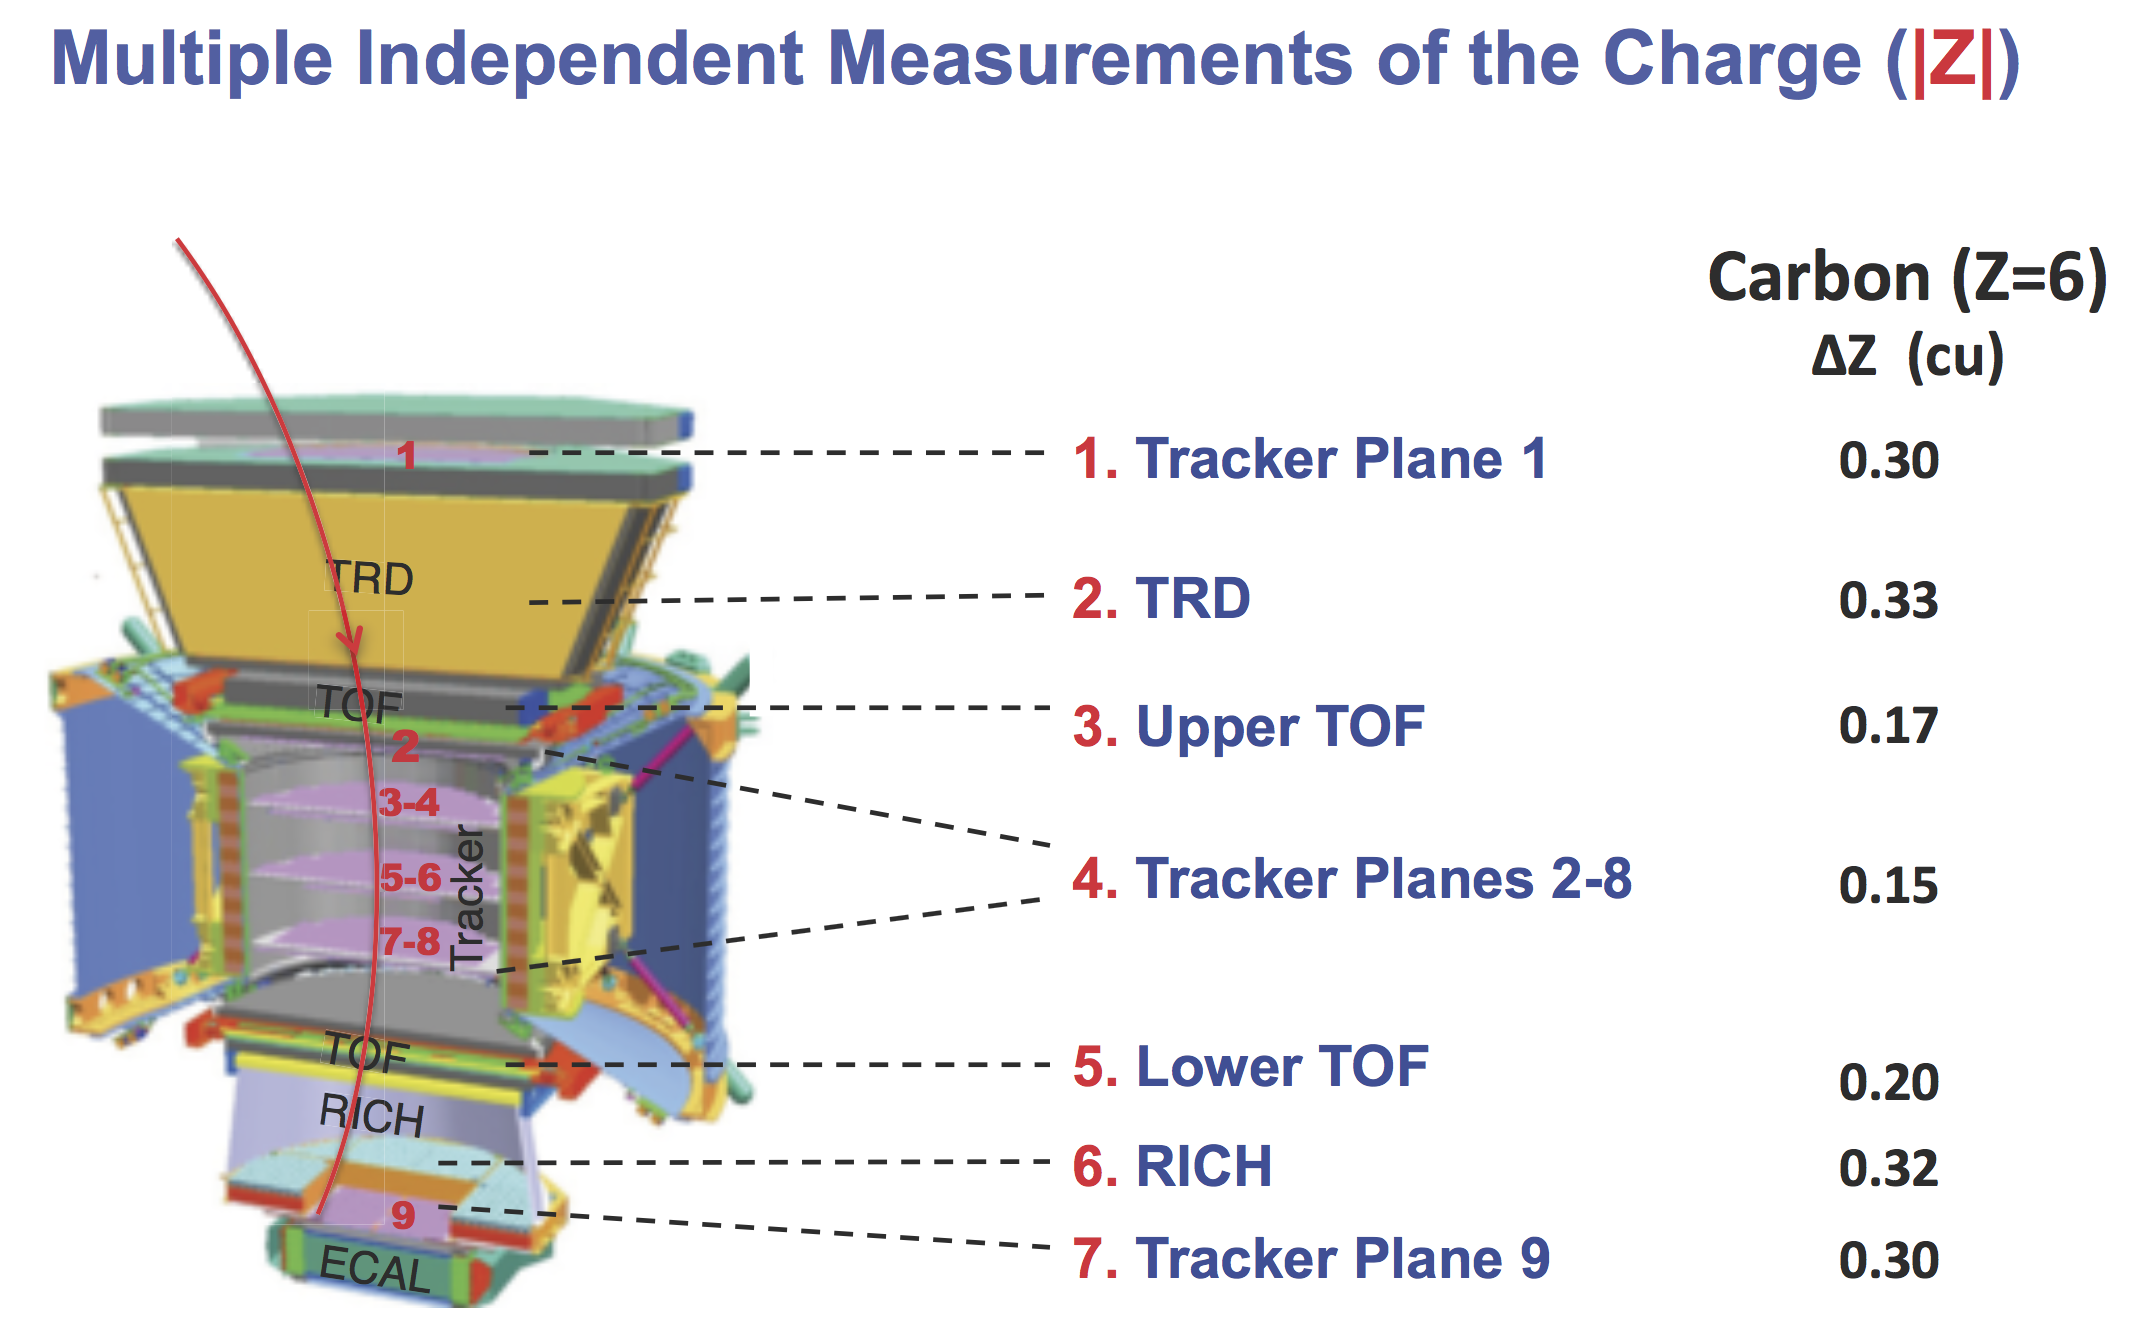
\includegraphics[height=0.55\paperheight]{Schem_Requirements-Charge02.png}
	\end{center}
\end{frame}

%\begin{frame}
%	\frametitle{Technical Requirement}
%	\framesubtitle{From the research on the Cosmic Ray}
%	\begin{center}
%		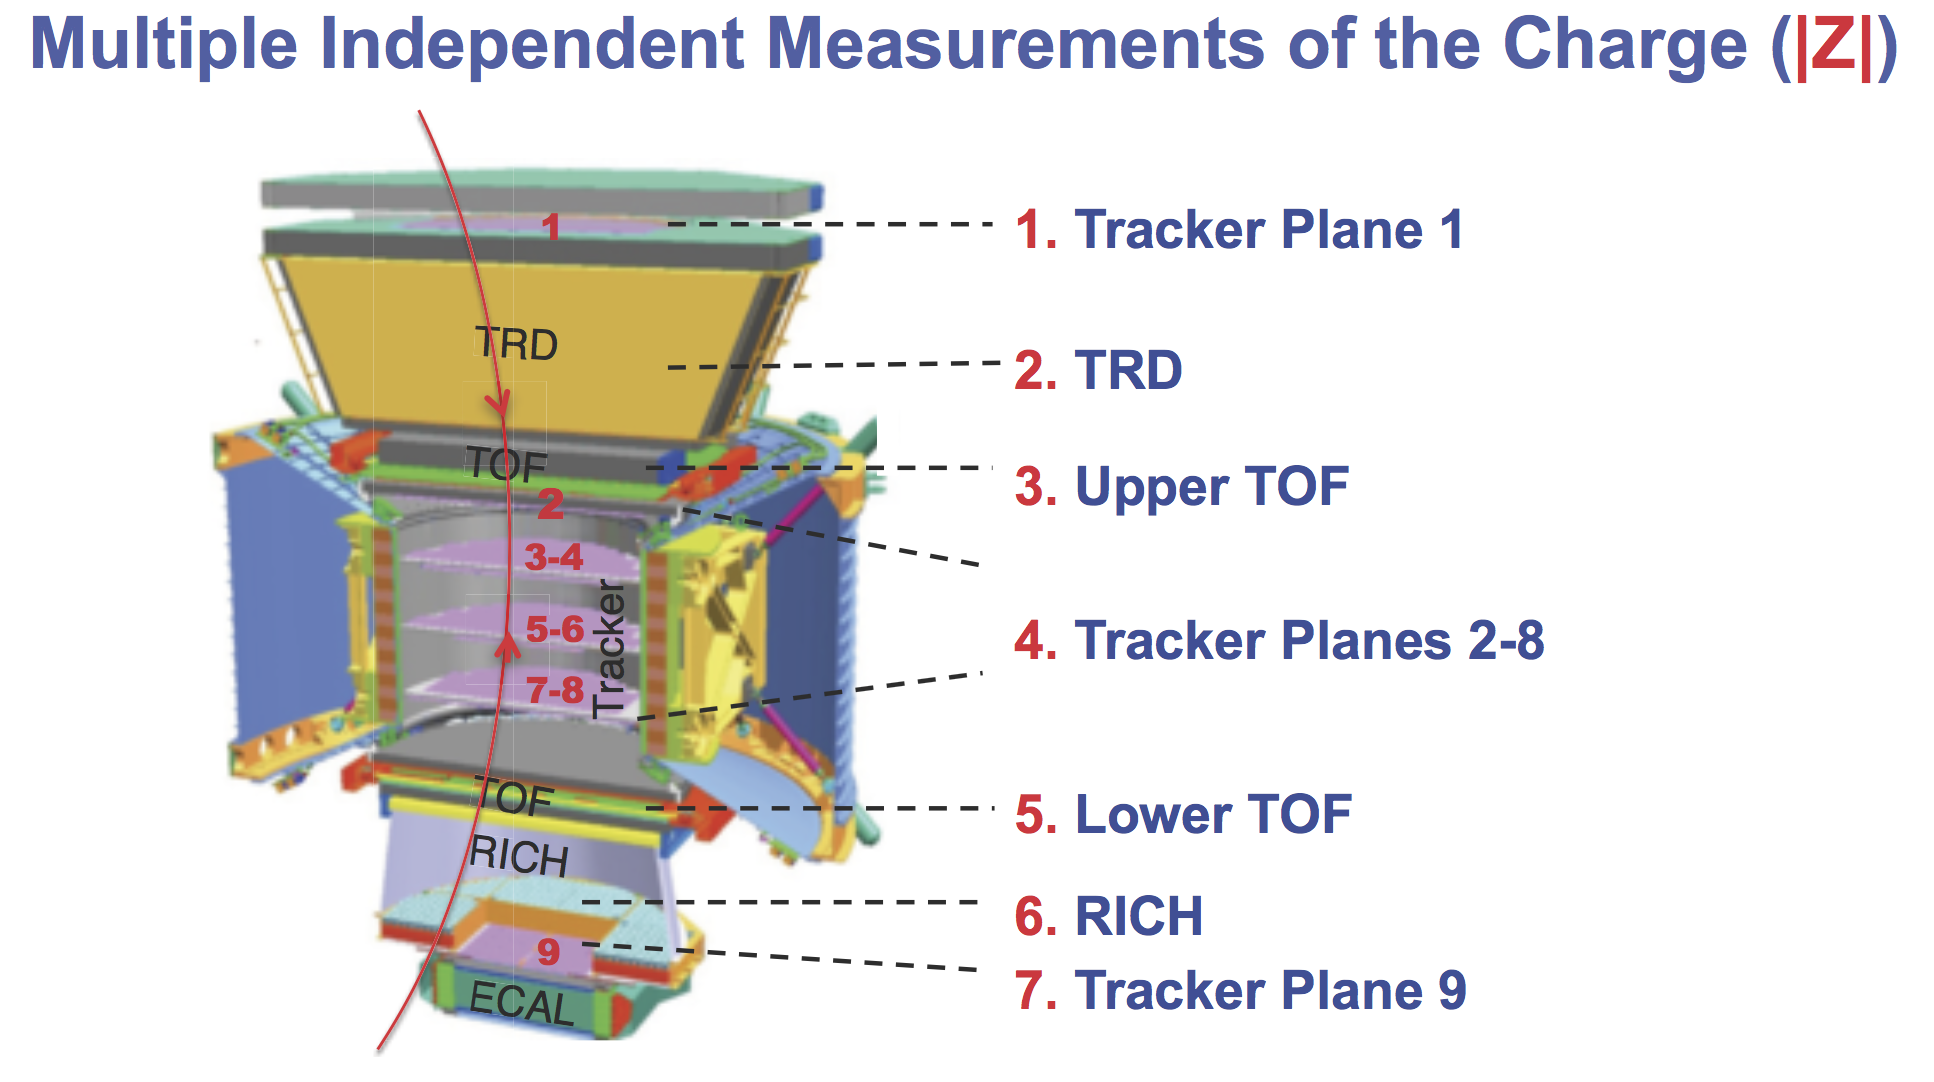
\includegraphics[height=0.5\paperheight]{Schem_Requirements-Charge.png}
%	\end{center}
%\end{frame}


\begin{frame}
	\frametitle{Technical Requirement} 
	\framesubtitle{From restriction of a space-borne experiment}
\end{frame}

\begin{frame}
	\frametitle{AMS-01} 
	\framesubtitle{The protype of AMS}
	%In order to ensure that technologies used in the detector construction work reliably in space, a scaled down detector 
	(AMS- 01) was built and flown in 1998 onboard the STS-91 mission for 10 days.
	Before installation on the Space Station, AMS performed an engineering flight on the Space Shuttle to ensure that:
	
	\begin{itemize}
		\item	The AMS experiment can function properly in space; in vacuum with orbital temperature changes from -65 to 40 
					$^{\circ}$C and in the intense radiation background (which contains heavy nuclei causing single event latch-up in 
					chips).
		\item	The detector can withstand the tremendous vibrations (150 dB) and acceleration (3 g) at launch and the 
					deacceleration (6.5 g) at landing;
	\end{itemize}

	This mission was subsequently referred to as AMS-01.
\end{frame}

\end{document}
